\section{Analisi dei problemi}
\epigraph{If we want machines to think, we need to teach them to see.}{\textit{Li Fei Fei}}
\subsection{Tecniche di computer vision}
La computer vision è un ambito dell'intelligenza artificiale il cui scopo è quello di insegnare alle macchine non solo a vedere un' immagine, ma anche a riconoscere gli elementi che la compongono in modo da poter interpretare il suo contenuto come farebbe il cervello di un qualsiasi essere umando. Nonostante le attuali tecniche di deep learning rendano possibile questo compito, è comunque necessaria una grande quantità di immagini e di tempo per poter allenare una rete neurale a sufficienza in modo da riuscire a riconoscere correttamente degli oggetti in un' immagine non incontrata durante il processo di allenamento.\\
L'obiettivo è quindi quello di riconoscere e classificare alcuni specifici elementi presenti in un'immagine localizzandone anche la posizione esatta all'interno dell'immagine stessa. Una volta trovata la sua locazione, l'oggetto viene messo in evidenza disegnando un rettangolo attorno ad esso, detto anche bounding box\gls, in modo che lo racchiuda con la maggiore precisione possibile. La classificazione ha invece come scopo quello individuare la categoria di appartenenza di un oggetto e la probabilità che essa sia realmente quella corretta.\\
Per classificare un singolo elemento in un'immagine viene tipicamente utilizzata una Convolutional Neural Networks (CNN)\cite{CNN} allenata con grandi quantità di immagini che possono essere tranquillamente reperite in rete già raggruppate in datasets come ad esempio ImageNet o Coco.\\
La vera sfida salta fuori non appena ci troviamo a dover riconoscere e classificare nella stessa immagine diversi oggetti appartenenti a categorie diverse, di differenti dimensioni e posizioni e talvolta anche sovrapposti. Questa è una situazione molto comune quando si ha a che fare con qualsiasi foto rappresentante il mondo reale. Il risultato ottimale sarebbe quindi di avere una bounding box di dimensioni corrette per ogni oggetto riconosciuto mostrando anche la categoria\gls di appartenenza dell'elemento insieme alla probabilità che la categoria predetta sia veramente quella corretta (detta anche score\gls). Per semplicità, la rappresentazione del bounding box di un elemento insieme alla sua categoria ed al suo score verrà chiamata label\gls
\begin{figure}[H]
	\centering
	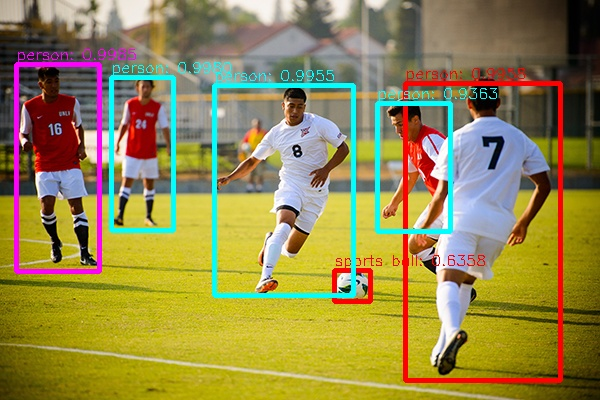
\includegraphics[width=0.7\linewidth]{images/esempio-detection.jpg}
	\caption{Esempio di un'immagine con box, categoria e probabilità per ogni elemento riconosciuto in essa}
	\label{Esempio di detection ideale}
\end{figure}
Per localizzare gli elementi, la tecnica più semplice consiste nel far scorrere una sliding window di varie dimensioni attraverso tutta l'area dell'immagine effettuando una classificazione per ogni locazione raggiunta. In caso di esito positivo la sliding window corrente corrisponderà al bounding box dell'oggetto classificato. Al termine del processo è possibile usare un algoritmo di non-max suppression (NMS) per rimuovere eventuali sovrapposizioni. Lo svantaggio di questo metodo è che bisognerebbe effettuare una detection per ogni sliding window comportando quindi un elevato costo computazionale. In particolare, nel caso di immagini in alta definizione si potrebbe addirittura arrivare ad avere migliaia di sliding windows comportando allo stesso tempo migliaia di detections per una sola immagine. Oltre al costo computazionale, questo metodo ha lo svantaggio di non sfruttare appieno la potenza di una rete neurale.\\
Per effettuare una detection, il metodo più utilizzato allo stato dell'arte è quello di utilizzare una R-CNN (Regional Convolutional Neural Network)\cite{RCNN} la quale sostituisce la tecnica della sliding window tramite un algoritmo greedy chiamato Selective Search che estrae dall'immagine delle regioni di interesse nelle quali è probabile che vi sia presente un oggetto. Queste regioni vengono poi date singolarmente in input ad una normale CNN la quale ha il compito di estrarne le caratteristiche principali per permettere ad una Support Vector Machine (SVM) presente nell'ultimo strato della CNN di rilevare la presenza di un oggetto ed eventualmente classificarlo.\\
Alternativamente, si possono prima utilizzare dei layers convoluzionali per estrarre una mappa delle caratteristiche più significative dall'immagine completa ed in seguito applicarci sopra un algoritmo di ricerca come Selective Search per trovare le regioni di interesse sulle quali effettuare la classificazione. Quest'ultimo metodo è conosciuto come Fast R-CNN\cite{fastRCNN} in quanto si ha un' efficienza maggiore rispetto a R-CNN per il fatto che l'operazione di convoluzione viene svolta solamente una volta per immagine invece che una volta per ogni regione di interesse.\\
Tuttavia, questi tipi di soluzioni presentano il difetto di richiedere molto tempo per eseguire l'operazione di ricerca delle regioni di interesse.\\
La versione più avanzata della Fast R-CNN ed attualmente in uso nei sistemi di computer vision attuali è chiamata Faster R-CNN\cite{fasterRCNN} e risolve il bottleneck della sua antecedente sostituendo la Selective Research con una Region Proposal Network (RPN). Essa prende come input un'immagine di qualsiasi dimensione e restituisce come output un insieme di rettangoli associati ad una probabilità che essi contengano un oggetto o meno. Come per Fast-CNN, viene prima effettuata una convoluzione per costruire la mappa delle caratteristiche più significative dell'immagine, in seguito viene utilizzata una sliding window per scorrere la mappa delle caratteristiche e darle in input a due fully-connected layers, dei quali, uno serve per individuare le coordinate del box dell'oggetto\footnote{Box-regression layer} mentre l'altro serve per ritornare la probabilità che nel box vi sia effettivamente un oggetto\footnote{Box-classification layer}. Infine queste regioni vengono passate ad un'altra rete che avrà come al solito il compito di riconoscere e classificare l'oggetto.
\subsection{Computer vision applicata su immagini ad alta risoluzione}
Sebbene sul web sia abbastanza facile reperire grandi quantità di immagini con cui allenare i propri modelli, tuttavia la maggior parte di questi datasets contiene solamente immagini a bassa risoluzione ed è difficile trovare in rete grandi datasets di immagini o video in alta risoluzione. Inoltre, la maggior parte dei modelli sono stati progettati per lavorare su immagini a bassa risoluzione (tra i 200 e i 600 pixels) sia per il fatto che una bassa risoluzione è comunque sufficiente per riconoscere e classificare un elemento, sia perchè è più efficiente lavorare su immagini di bassa qualità che su immagini con una risoluzione molto alta\cite{fasthighresolutiondetection}. In aggiunta, la maggior parte dei modelli esistenti tendono a ridurre automaticamente le dimensioni delle immagini troppo grandi per adattarle alla dimensione massima del proprio input\\
Lo svantaggio che questo comporta è che nelle immagini in bassa risoluzione si perdono molti dei dettagli che invece potrebbero essere catturati da un immagine o da un video ad alta risoluzione. In aggiunta, i video in 4K o addirittura 8K sono al giorno d'oggi sempre più diffusi, perciò anche gli attuali modelli dovranno prima o poi adattarsi per trattare efficacemente immagini di tali risoluzioni. Nella figura sottostante si può vedere un esempio di un frame in alta risoluzione nel quale, diminuendone le dimensioni e perdendo quindi qualità, non sarebbe stato possibile riconoscere alcune delle persone individuate nel frame.
\begin{figure}[H]
	\centering
	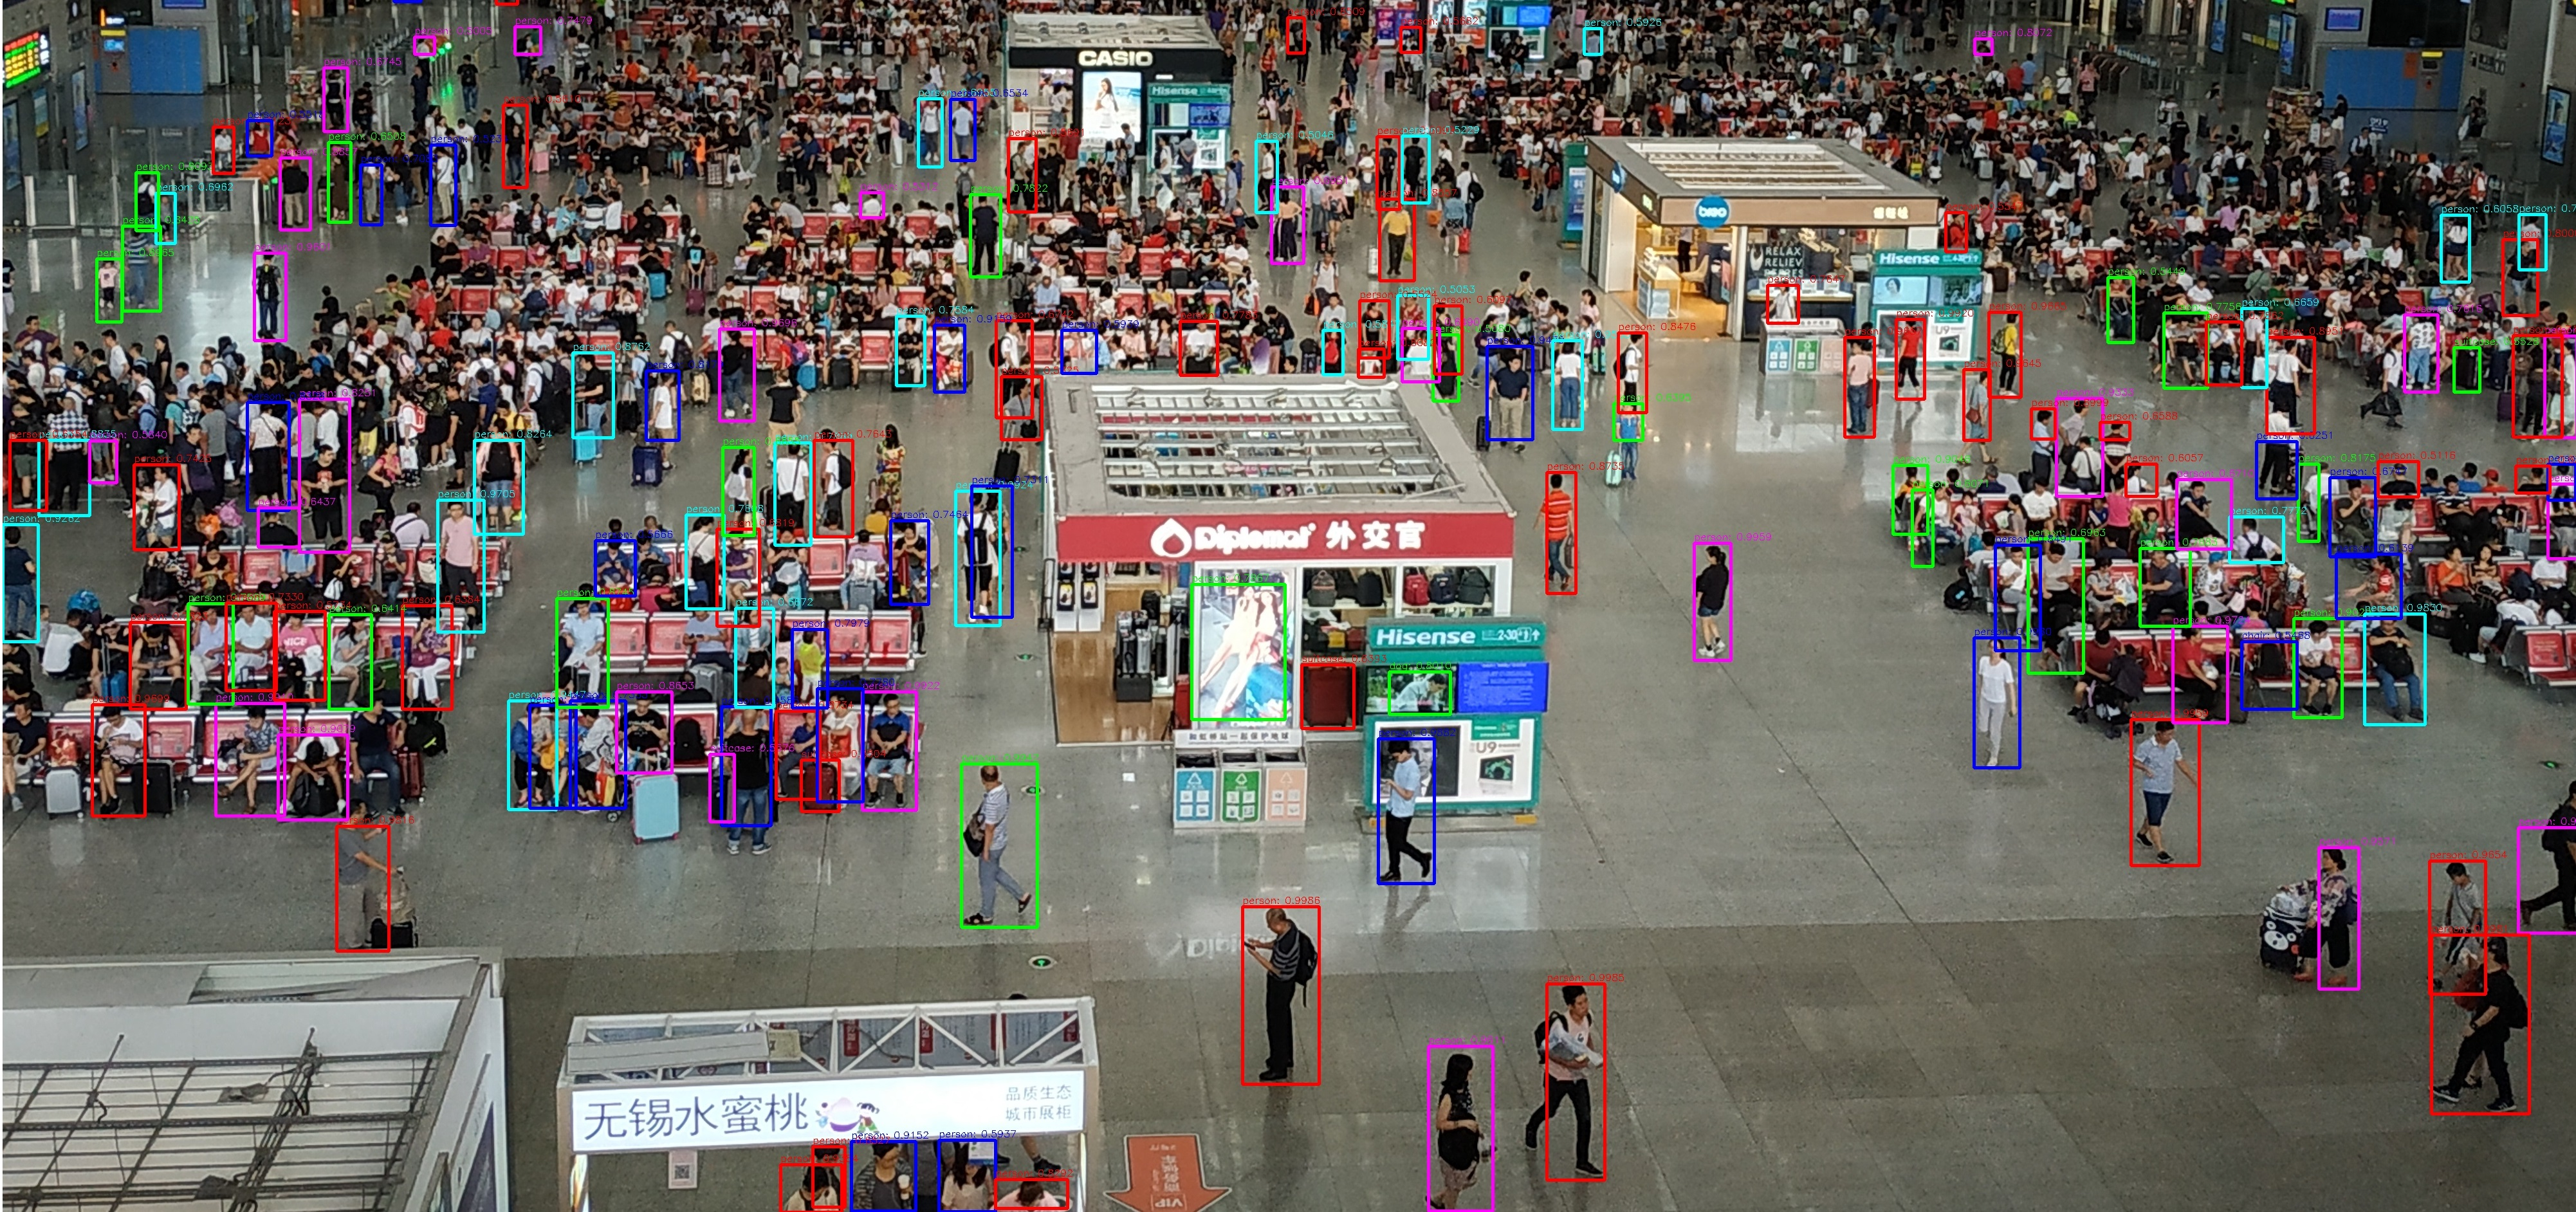
\includegraphics[width=0.7\linewidth]{images/immagine-4k.jpg}
	\caption{Esempio di object detection in un frame di un video in 4K}
	\label{Esempio di object detection in un frame di un video in 4K}
\end{figure}
\subsection{Frammentazione dell'immagine}
Per esempio, un'immagine in 4K ha una risoluzione di 3840 x 2160 pixels per un totale di 8294400 di pixels. Una rete neurale effettuerebbe un ridimensionamento dell'immagine per adattarla al meglio al suo input con conseguente perdita di risoluzione.\\ L'idea per aggirare il problema è quella di frammentare l'immagine in diverse sotto-immagini di dimensioni minori e quindi gestibili efficacemente da una singola rete neurale. Questa particolare strategia è chiamata frammentazione\gls dell'immagine e risulta essere molto utile in quanto permette di analizzare un'immagine ad alta risoluzione scomponendola in frammenti di dimensioni minori anziché gestirla nella sua interezza.
\begin{figure}[H]
	\centering
	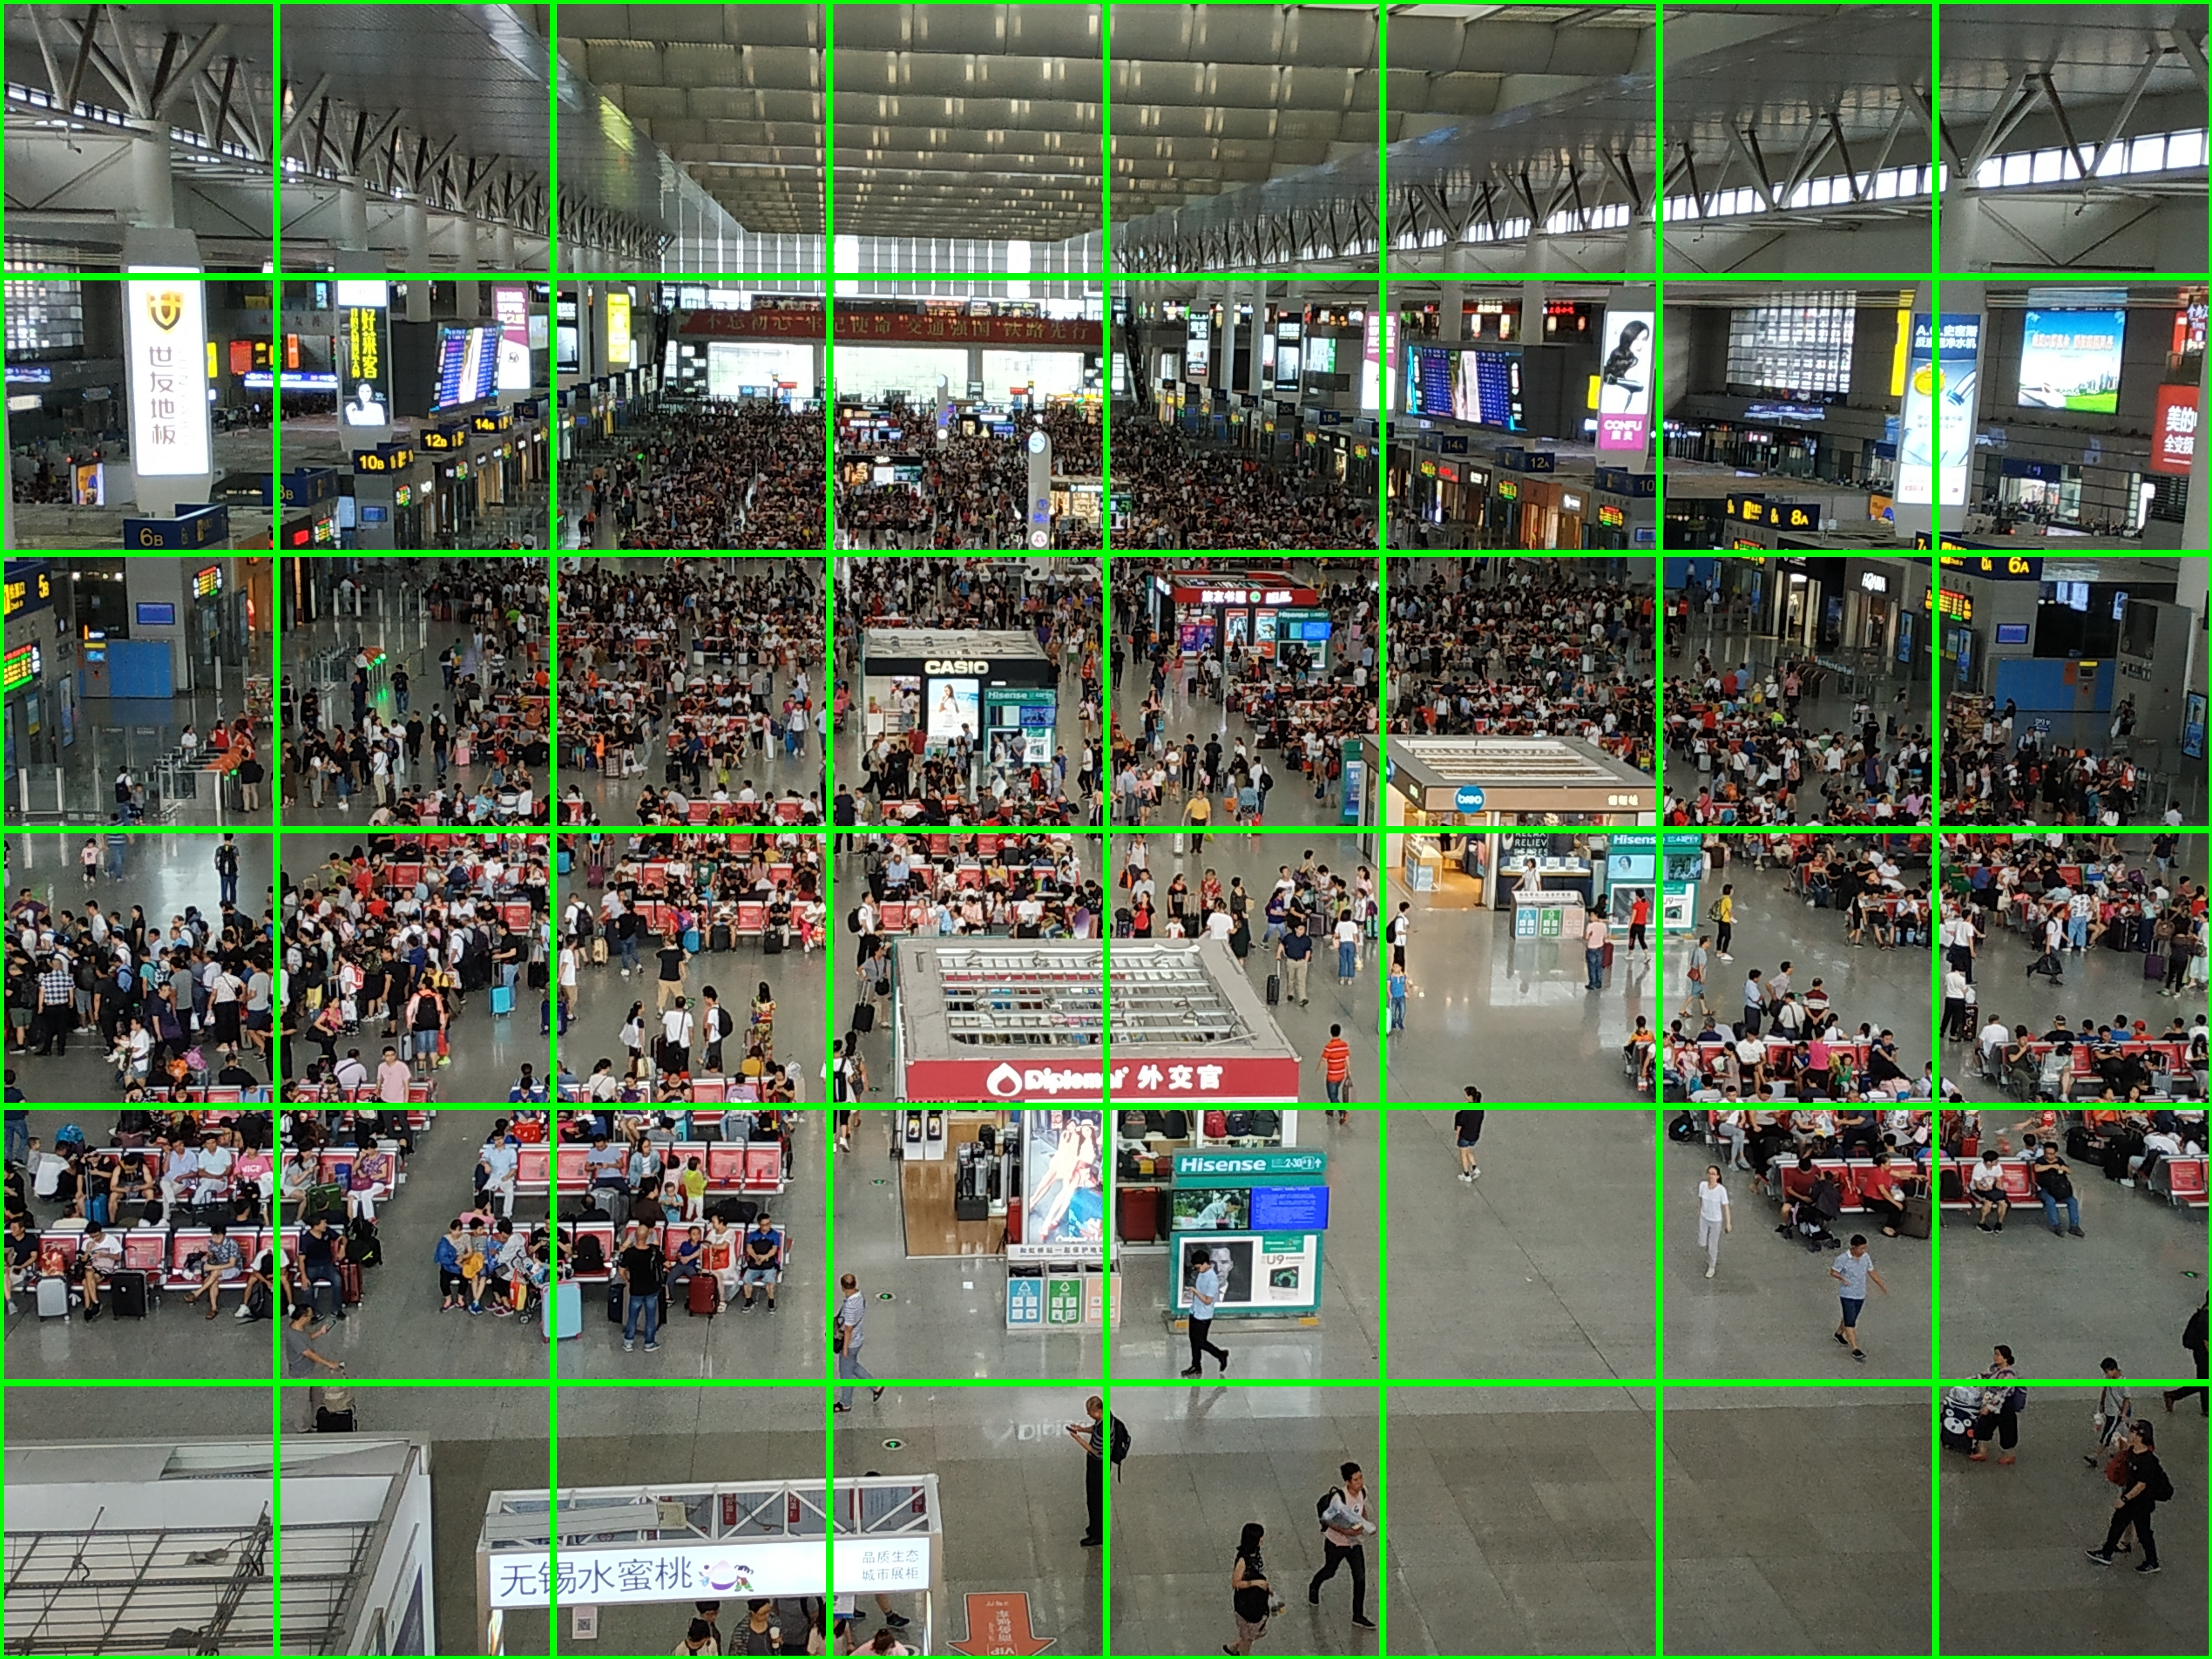
\includegraphics[width=0.5\linewidth]{images/esempio-frammentazione.jpg}
	\caption{Esempio di un'immagine in alta risoluzione suddivisa in regioni senza sovrapposizioni}
	\label{Esempio di un'immagine in alta risoluzione frammentata in regioni senza sovrapposizioni}
\end{figure}
Tuttavia questo procedimento non è esente da difficoltà.  Nel caso in cui un oggetto dovesse trovarsi su più regioni diverse, esso potrebbe venire identificato più volte o addirittura essere riconosciuto ogni volta come se fosse un oggetto appartenente ad una categoria diversa.\\
Un primo approccio per risolvere questo problema è quello di porre maggiore attenzione alle labels degli oggetti posizionati in prossimità dei confini delle regioni in quanto con molta probabilità è possibile che l'oggetto continui ad essere presente nella regione adiacente piuttosto che essere interamente contenuto nella regione esaminata. Se è quindi presente una label anche in una regione adiacente si passa allora alla verifica che le due label possano effettivamente appartenere allo stesso elemento. Per fare ciò bisogna assicurarsi che le due labels siano compatibili sia in termini di categoria che di posizione entro una certa soglia ed in caso affermativo fonderle in una sola label contenente l'oggetto intero.\\
Un' altra soluzione esaminata è quella di suddividere l'immagine intera in regioni con sovrapposizione il cui scopo è quello di generare intersezioni tra labels in prossimità dei confini migliorando al qualità delle detections nelle singole regioni. In questo modo un elemento contenuto all'interno di un'area di sovrapposizione tra più regioni genererebbe due o più labels parzialmente sovrapposte.\\
Nel caso in cui l'area di sovrapposizione dovesse essere più consistente, il problema può essere facilmente gestito con un algoritmo di non-max suppression, il quale, per ogni insieme di labels parzialmente sovrapposte e con stessa categoria, tende ad eliminare le labels con probabilità minore tenendo valida solo quella con probabilità massima.\\
Tuttavia, il caso più insidioso ed allo stesso tempo più frequente lo si ha quanto due labels sono solo leggermente sovrapposte: la prima difficoltà la si ha nel decidere se procedere ad unificarle in una sola label o meno, la seconda riguarda quale criterio utilizzare per effettuare la loro unione. E' proprio per far fronte a questi problemi che è stato ideato ed implementato un algoritmo il quale verrà descritto nella \textit{sezione 4.1}.
\subsection{Tecniche di object tracking}
Il tracciamento di oggetti in un video è uno di quei problemi presenti nell'ambito dell'informatica che non sono ancora stati risolti ottenendo risultati soddisfacenti. Il tracciamento consiste non solo nel localizzare e tracciare degli oggetti di interesse attraverso una sequenza di frames ma anche nel riconoscere che l'oggetto tracciato è sempre lo stesso.\\ 
Il problema non è per niente banale se pensiamo che in un video uno stesso oggetto può spostarsi, nascondersi dietro qualche altro elemento, deformarsi, risultare sfocato, cambiare le sue dimensioni, la sua illuminazione, la sua velocità ed il tipo di background. Nel caso ancora peggiore un oggetto tracciato potrebbe addirittura scomparire in un frame per poi ripresentarsi solamente dopo che sono trascorsi un numero casuale di frames.\\
Un algoritmo di tracking ottimale dovrebbe essere in grado di far fronte a tutti questi problemi riconoscendo quindi gli oggetti da esso tracciati tramite per esempio l'assegnazione di un ID univoco.\\ 
Una possibile soluzione per affrontare questo problema consiste nell'eseguire inizialmente una normale detection sul primo frame del video in modo tale da individuarne tutti gli elementi presenti e le rispettive labels. In seguito, ognuno di questi elementi viene assegnato ad un tracker\gls che avrà il compito di tracciare l'elemento nei frames successivi.\\ 
Tracciare un elemento è un' operazione meno onerosa rispetto alla sua individuazione in quanto il tracker conosce già alcune informazioni relative all'oggetto tracciato, acquisite nei frames precedenti, potendo così tenere in memoria uno storico del suo stato, come per esempio, le sue ultime locazioni. Per aumentare la sua precisione, un tracker non tiene conto solamente della locazione dell'elemento osservato ma può anche tenere memoria di altre utili informazioni aggiuntive come la sua direzione, la sua velocità, le sue dimensioni, una previsione delle locazioni future analizzandone la sua traiettoria oppure può memorizzare un hash\footnote{Al contrario degli hash usati in crittografia, un hash applicato alle immagini è progettato in modo tale che piccole variazioni dei pixels dell'immagine non risultino in un hash molto diverso da quello originale} dei pixels presenti all'interno del bounding box dell'oggetto per poi confrontarlo con l'hash dello stesso oggetto calcolato nel frame successivo\cite{imagehash}.\\
I trackers più performanti come CSK, MOSSE\cite{mosse} e GOTURN\cite{goturn} utilizzano alcune delle informazioni sopra descritte per costruire un filtro di correlazione in modo da localizzare l'oggetto nel frame successivo e migliorare la precisione del filtro con le successive individuazioni. Lo scopo del filtro è quindi quello di minimizzare la differenza tra l'output predetto e quello originale.\\ Nonostante tutti questi accorgimenti è però inevitabile che col trascorrere dei frames i trackers cominceranno ad essere sempre più imprecisi nell'individuare il loro oggetto tracciato. In particolare, questa situazione può accadere molto velocemente in quei video dove avvengono molti spostamenti e sovrapposizioni tra elementi. Inoltre, ad un certo frame del video è possibile che si presentino nuovi elementi o che ne scompaiano alcuni. E' quindi buona norma aggiornare i trackers con le locazioni corrette dei loro elementi tracciati, creare nuovi trackers per ogni nuovo elemento e cancellare i trackers per gli oggetti spariti effettuando una nuova detection ogni fissato numero di frames.\\
E' qui che si presenta il problema di maggiore rilevanza: una nuova detection effettuata su un nuovo frame non tiene conto delle informazioni acquisite in precedenza in quanto queste con molta probabilità risulterebbero errate o imprecise. Il problema è quindi quello di riassegnare a ciascun oggetto individuato lo stesso ID che possedeva in precedenza ed assegnare un nuovo ID ad ogni oggetto comparso nel video per la prima volta.
\begin{figure}[H]
	\centering
	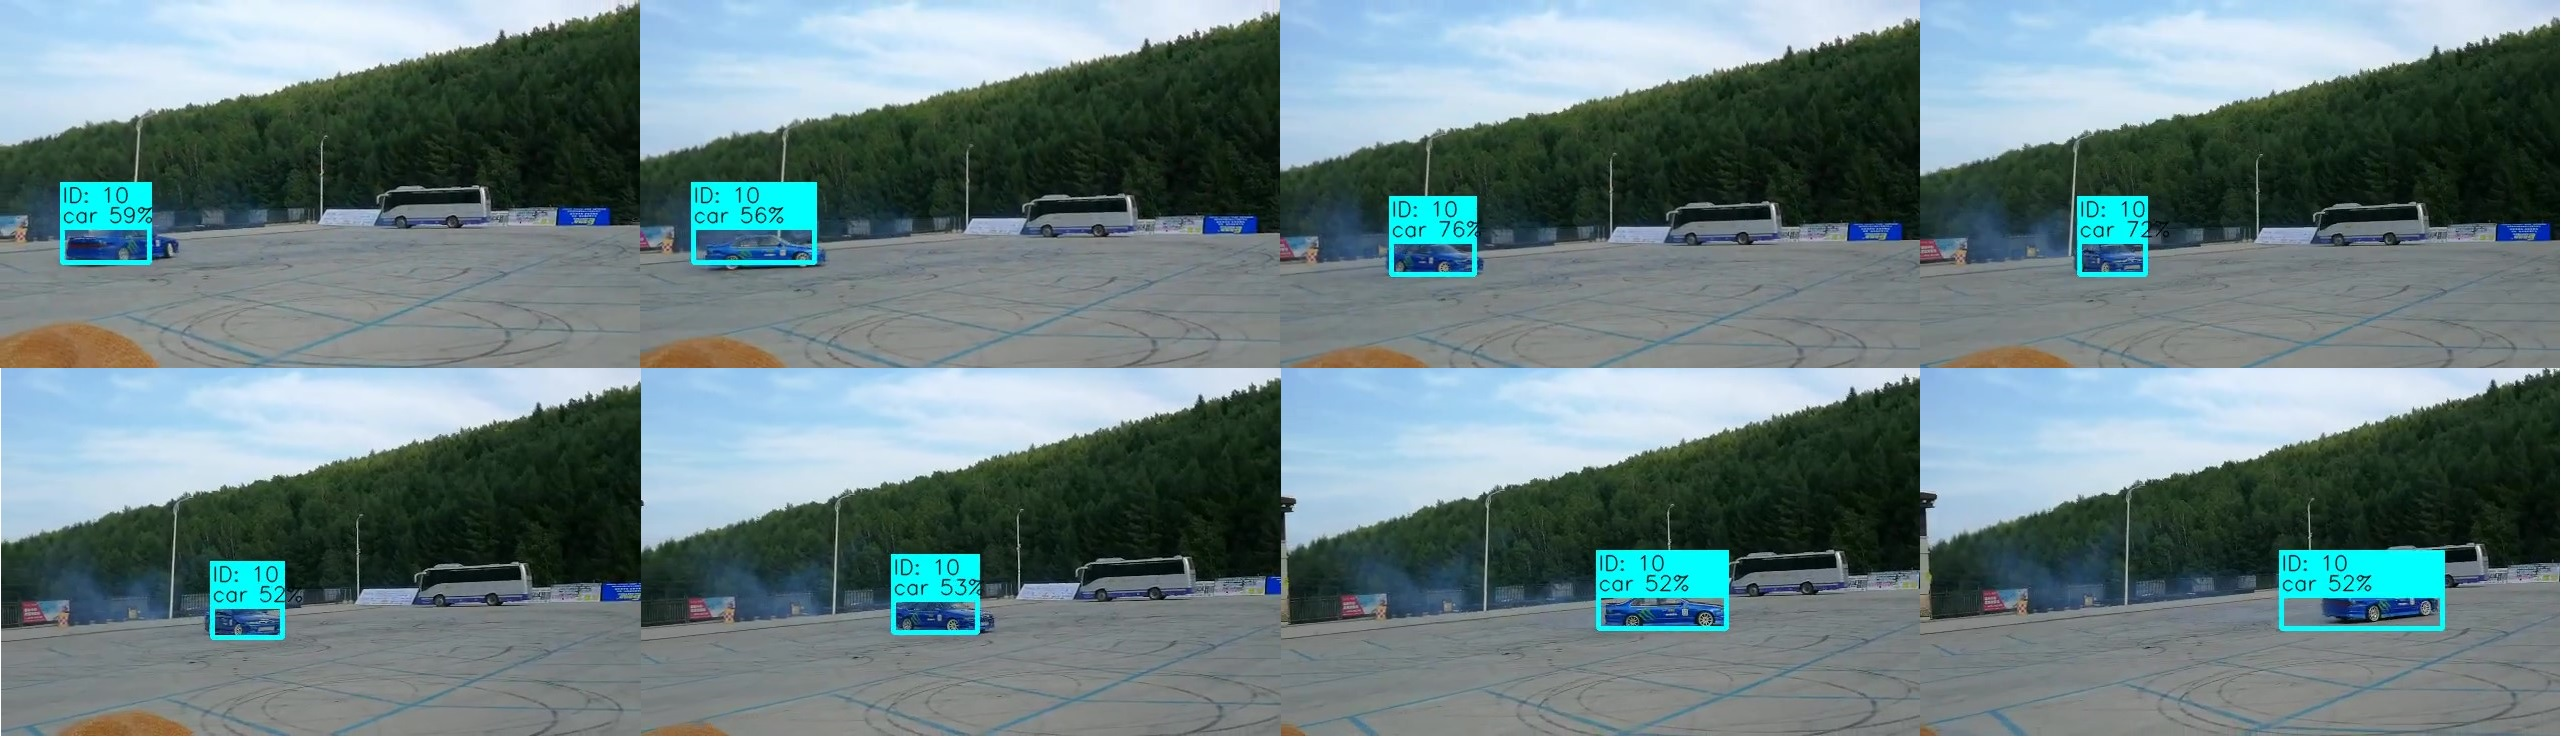
\includegraphics[width=1\linewidth]{images/esempio-tracking.jpg}
	\caption{Frames di un video nei quali viene tracciata un' auto (ordinati da sinistra a destra e dall'alto al basso)}
	\label{Esempio di un'immagine in alta risoluzione frammentata in regioni senza sovrapposizioni}
\end{figure}
\subsection{Object tracking con continue object detections}
Considerata la scarsa affidabilità degli attuali algoritmi di tracciamento, nella soluzione individuata gli oggetti vengono identificati effettuando una nuova detection per ogni frame del video in modo da assicurarsi di avere sempre una buona accuratezza ed allo stesso tempo migliorare l'efficacia dei trackers migliorando gradualmente la precisione dei loro filtri di predizione. Questo metodo sacrifica l'efficienza del processo per migliorarne l'efficacia. A meno che non venga utilizzato un algoritmo di detection molto veloce come SSD (Single Shot Detector)\cite{ssd} non è possibile applicare il tracking sui video in tempo reale in quanto il frame rate che ne risulterebbe sarebbe troppo basso. A seguito di una nuova detection, per effettuare una corretta riassegnazione degli ID viene fatto un confronto tra le labels presenti nel frame precedente con quelle presenti nel frame corrente con lo scopo di trovare una corrispondenza biunivoca tra due labels e capire quando entrambe si riferiscono allo stesso elemento in modo da garantire un corretto trasferimento dell'ID. Per rendere tutto ciò possibile viene utilizzato un filtro in grado di predire le locazioni future di un oggetto tenendo traccia dei suoi bounding boxes e poi correggersi tramite misurazioni successive. Anche per realizzare questa soluzione è stato ideato ed implementato un algoritmo descritto nella \textit{sezione 4.2}.
